\documentclass[journal, a4paper]{IEEEtran}

%\usepackage{cite}
\usepackage{graphicx}
%\usepackage{psfrag}
%\usepackage{subfigure}
\usepackage{url}
%\usepackage{stfloats}
\usepackage{amsmath}
%\usepackage{array}
\usepackage{gensymb}

% Package Settings
\graphicspath{ {../images/} }

\begin{document}

% Define document title and author
\title{Testing the Effects of Transfection on Mammalian Cytokine RNA Expression}
\author{Austin Mitchell Vecchio
\thanks{Advisor: Dipl.--Ing.~Michelle Ammerman, Lehrstuhl f\"ur Nachrichtentechnik, TUM, WS 2050/2051.}}
\maketitle

% Write abstract here
\begin{abstract}
  Abstract outline

  This experiment aims to study the effect of genetic expression on polyplex treated cells against $\beta$-actin and INF$\alpha$.

\end{abstract}

% Each section begins with a \section{title} command
\section{Introduction}
  \PARstart{G}{ene} therapy is an experimental method for treating disease by introducing a healthy copy of a
  defective gene into the patient's cells to alter the patients genetic material.
  The alternative is a non viral gene therapy method which can often have simple and large scale production
  with low host immunogenicity. However, non viral gene therapy can often yield low transfection efficiencies.
  This low yield is often due to The inate immune response. The inate immune response to foreign DNA (often by viruses or bacteria) through cytokines
  as a trigger that rejects the foreign DNA through one of three possibilities. These possibilities include: inducing
  cell death, halting the production of protien or recruiting immune cells to initiate an adaptive immune response (e.g. antibody protection).
  New advances in technologies have improved transfection efficiency by modifying cytokines. Cytokines
  are small protiens that are involved in various types of cell signaling. Classifications of these signalings
  include interferos, chemokines and interleukins.
  This experiment aims to see if the inate immune response can be inhibited or manipulated to improve gene therapy treatments.

  In this experiment, the prostate cell line will be used for the transfection of foreign DNA. Prostate cells provide a glandular function
  in the body by generating fluid which serves several functions in reproduction. The analysis will focus on quantifying foreign mRNA that will be
  produced from the prostate cells. This process will be carried out by nanoparticles that are formed by the self-assembly of DNA/RNA and cationic polymers
  called polyplexes. Polyplexes are specifically designed to deliver foreign genetic material to cells by a process called transfection.
  
  There are two devices used in this experiment. The first device, the Qubit, is an electronic device that quantifies a substance through fluorescence.
  The second device is qPCR.
  Reverse Transcriptase (RT)qPCR is a technique used to describe the level of genetic expression is occuring in vitro
  by measuring the amount of mRNA within a sample. In this technique, mRNA is reverse transcribed in to complementary DNA by
  an enzyme labeled reverse transcriptase.
  For the Real Time PCR experiment, since it is impossible to eliminate all genomic DNA from the cDNA synthesis, two solutions will be prepared.
  The first solution will be a +RT which will include reverse transcriptase and thus, will have cDNA.
  The second solution will be a -RT solution which will lack reverse transcriptase.
  When QtPCR is performed on the -RT solution, genomic DNA will be amplified and will be seen in the resulting data.
  In this experiment, $\beta$-actin and RPL13A will be used for direct controls against the immunological transcripts.
  INF$\beta$ will not be used as it will only appear after cycle 40 in the experiment producing undesirable results.
  The No Template Control will consist of DEPC water.
  The immunological transcripts that will be used in this experiment are Interleukin-6 (IL6) and Inferon-$\alpha$ (INF$\alpha$)
  Beta actin is a type of actin isoform which is highly involved in cell motility, structure and integrity.
  RPL13A is a gene that codes for the 60S ribosomal L13a protein.
  Interleukin-6 (IL-6) is a multifunctional cytokine that defends the host in response to immune and hematopoietic activities.
  Interferon-$\alpha$ is a part of a large subgroup of interferon protiens that help regulate the activity of the immune system.

\section{Methods}
    \subsection{RNA Purification}
      The cells in trizol were thawed before phase separation. During phase separation,
      the poly treated cells in trizol were incubated at 42$^{\circ}$ after which an 0.2mL of chloroform was added per 1mL of Trizol.
      The homoginized sample was incubated at 42$^{\circ}$ for 2-3 minutes following a vigorous shake for 15 seconds.
      The sample was then centrifuged 12,000 g for 15 minutes at 4$^{\circ}$C before transfering the aqueous phase
      to a second tube. (100%) 0.5mL Isopropanol was added to the aqueous phase per 1mL of Trizol used.
      Again, the sample was centrifuged 12,000 g for 15 minutes at 4$^{\circ}$C.
      The pellet was not washed in fear of losing RNA.
      The solution then, underwent a series of centrifuges in between the removal of ethanol to result in an RNA pellet.
      The pellet was then air dried to remove remaining ethanol.
      The pellet was incubated at 42$^{\circ}$ following a resuspension in 20$\mu$L of RNase free water.

    \subsection{cDNA Synthesis}
      For the first step of cDNA Synthesis, two solutions (+RT/-RT) were formed from the following compounds:
      10x dsDNase Buffer, dsDNase, Template RNA, polyplex 24hour RNA and nuclease free water.
      Both solutions were incubated at 42$^{\circ}$ after being centrifuged. The solutions were then chilled on ice, centrifuged and placed back on ice.
      For both solutions, 5X Reaction mix and nuclease free water was added. In the +RT solution, Maxima Enzyme mix (reverse transcriptase) was added to the mixture.
      The -RT solution used DEPC H20 instead of Maxima Enzyme mix so that the -RT solution can simulate the +RT solution without synthesizing RNA into cDNA.
      When the -RT solution undergoes QtPCR, any contaminating genomic DNA will be amplified.
      The two solutions will be then mixed gently and centrifuged. An incubation period will take place at 25$^{\circ}$C for 10 min
      followed by a second incubation session at 50$^{\circ}$C for 15 min.
      The reaction will be terminated by heating the solutions at 85$^{\circ}$C for 5 min.
      This process was conducted using Maxima First Strand cDNA Synthesis Kit with dsDNase (Thermo Scientific, Cat#: K1671)

    \subsection{Qt PCR}
      Each well will contain 10$mu$L of 2X iTaq universal SYBR Green Supermix,
      5$\mu$L of a primer (IL6, INF$\alpha$, $\beta$-actin or RPL13A),
      and 5$\mu$L of the respective diluted cDNA.
      The cDNA needs to be diluted to 4ng/$\mu$L from their respective concentrations before it is added to the wells.
      The concentrations of cDNA for both sets of Poly24 and no washed cells were all around 100ng/ $\mu$ L.
      Therefore only one set of calculations were needed for determining the proper dilution of cDNA into water
      for either INF$\alpha$ and IL6 or $\beta$-actin andRPL13A and the respective -RT wells. For just cells,
      a different set of calculations were needed since the original cDNA concentrations were around 11 ng/ $\mu$ L.
      All wells contained the Green Supermix. The columns were sorted in the following manner:
      1-3 contained IL6, 4-6 contained INF$\alpha$, 7-9 contained $\beta$-acting and 10-12 contained RPL13A.
      Refer to Table II for a compressed map of the PCR wells. The QtPCR was ran for 40 cycles.

    \subsection{Gel Electrophoresis}
      In order to further understand the results gained from the QtPCR, an 1.2% agarose gel was poured
      and gel electrophoresis was ran on the PCR product.

    \subsection{Analysis}
      The results from the QtPCR produced Ct values from each well.
      A Ct value is a numeric inverse correlation to the quantity of nucleic acid detected by the aparatus.
      Comparisons are made between Polyplex treated cells for 24 hours version [AV], Polyplex treated cells for 24 hours version [Ts],
      Polyplex treated cells for 6 hours with iCRT, Cells that were not washed after 6 hours, cells that were not washed and just cells.
      Each comparison was conducted by taking the difference between the Ct values of the two primers (immunological transcript minus control)
      on two different treatments. A second difference was taken between these two treatments (i.e. Poly24-NoWash) and then applied to the $\Delta$\Delta$ct method
      to determine the fold induction. This was repeated three times, and thus an average was determined.

\section{Results}

  \subsection{Qubit}
    Following the cDNA synthesis, the concentrations were measured by the Qubit. The concentrations are as follows:
    SD1 (standard 1): 54.27ng/$\mu$L, SD2 (standard 2): 1057.52ng/$\mu$L, Tk: 8.75ng/$\mu$L,
    DA: 68.0ng/$\mu$L, AV: 487.0ng/$\mu$L, Ts: 28.0ng/$\mu$L.

  \subsection{QtPCR}

    \begin{table}[!hbt]
      % Center the table
      \begin{center}
      % Fold Inductions
      \caption{Wells for Immunological Responses}
      \label{tab:simParameters}
      % Table itself: here we have two columns which are centered and have lines to the left, right and in the middle: |c|c|
      \begin{tabular}{|c|c|c|c|c|}
        \hline
        & IL6 & INF$\alpha$ & $\beta$-actin & RPL13A \\
        \hline
        Poly24[AV]-NoWash & 3.85E-05 & 7.58E-03 & 5.09E-05 & 1.05E-02 \\
        \hline
        Poly24[AV]-Cells & 3.10E-02 & 3.54E-02 & 3.94E-02 & 4.27E-02 \\
        \hline
        NoWash-Cells & 8.01E+02 & 4.65E+00 & 7.01E+02 & 4.08E+00 \\
        \hline
        Poly24[Ts]-NoWash & 8.20E-05 & 4.64E-03 & 3.77E-05 & 6.04E-03\\
        \hline
        Poly24[Ts]-Cells & 6.54E-02 & 5.90E-02 & 2.57E-02 & 2.55E-02\\
        \hline
        Poly6+iCRT-NoWash6 & 5.00E+2 & 4.21E+2 & 2.58E+1 & 2.23E+1 \\
        \hline
      \end{tabular}
      \end{center}
    \end{table}

  \subsection{Gel Electrophoresis}

    \begin{figure}[t]
      \centering
      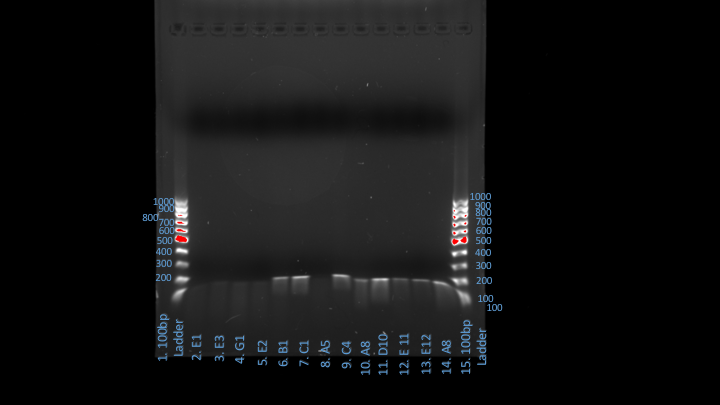
\includegraphics[width=8cm]{supergel}
      \caption{A 1.2\% agarose gel used to further analyze discrepencies seen in the melt curves of the PCR product.}
      \label{fig:mesh1}
    \end{figure}

    Refering to Figure 1, it can be seen that the selections of PCR products was based off of melt curves that were inconsistent with
    surrounding wells of similar product (i.e. $\beta$-actin for just cells).
    Lanes 2-4 (Wells: E1,E2,E3,G1) consists of -RT solutions. These lanes are empty displaying
    genomic DNA that is almost undetectable. Lane 8 (Well A5) displays a lack of cDNA
    for Interferon-$\alpha$ where there should exist amplified cDNA. Lanes  7,9,11 and 14
    (Wells: C1,C4,D10,A8) are displaying bands at a greater illumination compared to other lanes.
    Lanes 7 and 9 consist of Just Cells in Interleukin-6 and Interferon-$\alpha$ respectively.
    Lanes 11 and 14 are polyplex cells treated for a 24 hour duration in both the [AV] and [Ts] variants
    for RPL13A and $\beta$-actin respectively.
    Lanes 6,12, and 13 contain smaller amounts of cDNA compared to Lanes 7,9,11 and 14 as they do not contain
    as great illumination.
    Lane 6 (Well B1) is cells that were not washed for Interleukin 6.
    Lanes 12 and 13 (Wells: E11,E12) consist of -RT solutions for RPL13A displaying amplified genomic DNA.

\section{Discussion}

The mRNA was purified and converted to cDNA. THe resulting concentration was relatively high compared to peers. This eludes that the
treatment for these cells of polycationic DNA for 24 hours could result in higher transcription rates.

\section{Conclusion}

To futher understand the nature polyplex treated cells in response to a specific duration,
it would be suggested that the polyplex cells are treated in 3 hour increments from 3 hours to 24 hours.


\section{Figures}

  \begin{table}[!hbt]
    % Center the table
    \begin{center}
    % Fold Inductions
    \caption{PCR Wells for Controls}
    \label{tab:simParameters}
    % Table itself: here we have two columns which are centered and have lines to the left, right and in the middle: |c|c|
    \begin{tabular}{|c|c|c|c|c|c|c|c|c|c|c|c|c|c|}
      \hline
      & Primer & 1/4/7/10 & 2/5/8/11 & 3/6/9/12 \\
      \hline
      A & Poly24[Tk] & 4ng/$\mu$L & 4ng/$\mu$L & 4ng/$\mu$L\\
      \hline
      B & Just Cells & 4ng/$\mu$L & 4ng/$\mu$L & 4ng/$\mu$L\\
      \hline
      C & No Wash & 4ng/$\mu$L & 4ng/$\mu$L & 4ng/$\mu$L\\
      \hline
      D & Poly24[AV] & 4ng/$\mu$L & 4ng/$\mu$L & 4ng/$\mu$L\\
      \hline
      E & -RT & Poly24[Tk] & Cells & Poly24[AV] \\
      \hline
      E & NTC & Poly24[Tk] & Cells & Poly24[AV] \\
      \hline
      G & & NoWash(-RT) & NoWash(NTC) &\\
      \hline
      H & & & &\\
      \hline
    \end{tabular}
    \end{center}
  \end{table}

  \begin{table}[!hbt]
    % Center the table
    \begin{center}
    % Fold Inductions
    \caption{List of Primers}
    \label{tab:simParameters}
    % Table itself: here we have two columns which are centered and have lines to the left, right and in the middle: |c|c|
    \begin{tabular}{|c|c|c|}
      \hline
      Primer Name & Tm & Sequence \\
      RTPCR-IL6-FOR & 60 & CCTTCCAAAGATGGCTGAAA \\
      \hline
      RTPCR-IL6-REV & 60 & CACAGCTCTGGCTTGTTCCT \\
      \hline
      RTPCR-IFNAall-FOR & 61 & GCACCGAACTCTACCAGCAG \\
      \hline
      RTPCR-IFNAall-REV & 60 & ACAACCTCCCAGGCACAA \\
      \hline
      RTPCR-B-Actin-FOR & & TTGCCGACAGGATGCAGAA \\
      \hline
      RTPCR-B-Actin-REV & & GCCGATCCACACGGAGTACTT \\
      \hline
      RTPCR RPL13A –FWD & & CCTGGAGGAGAAGAGGAAAGAGA \\
      \hline
      RTPCR RPL13A REV & & TTGAGGACCTCTGTGTATTTGTCAA \\
      \hline
    \end{tabular}
    \end{center}
  \end{table}

  \begin{figure}[t]
    \centering
    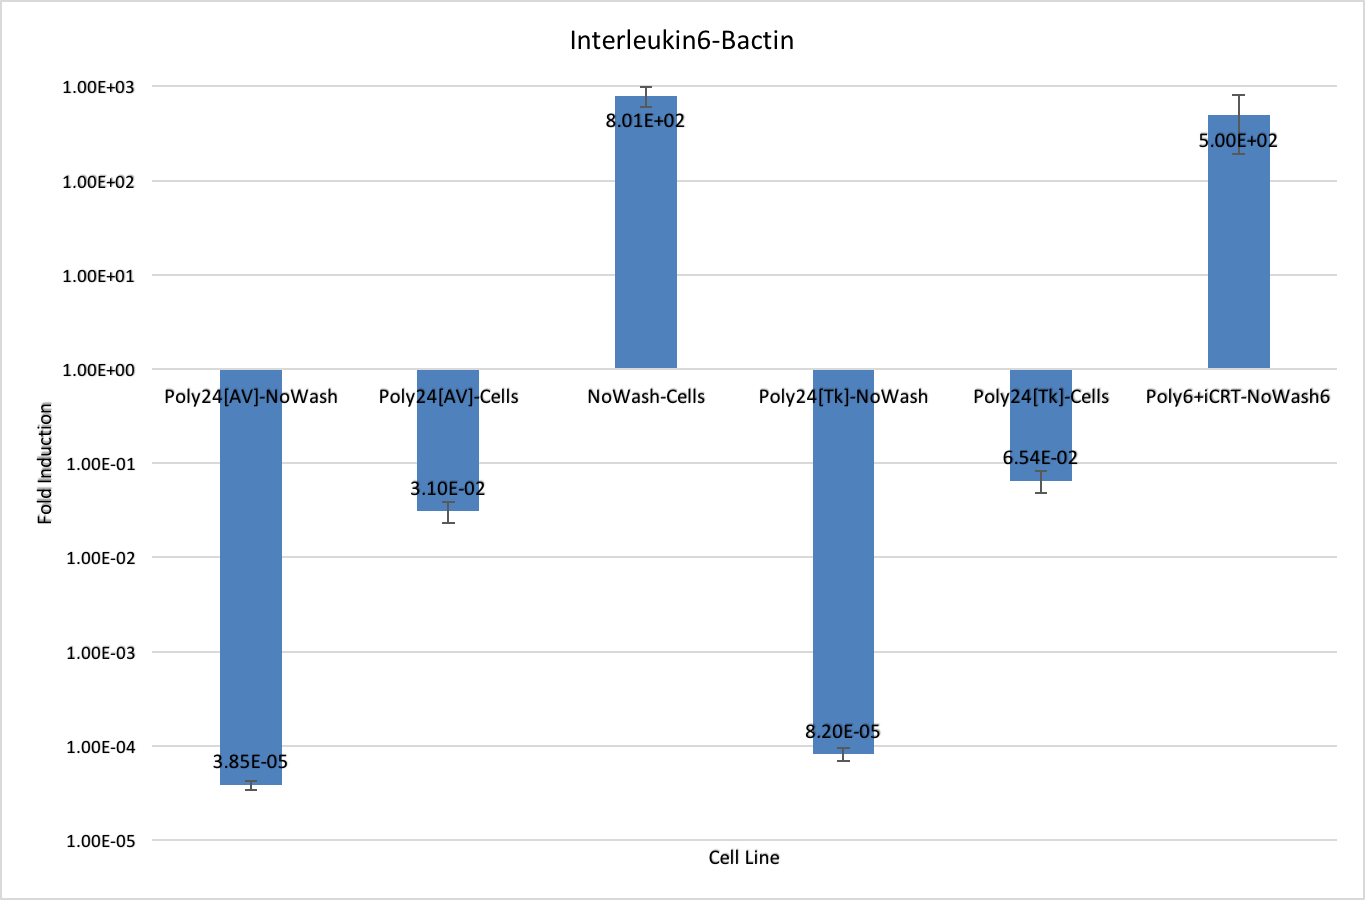
\includegraphics[width=8cm]{il6-bactin}
    \caption{Logarithmic fold Inductions for Interleukin-6 vs $\beta$-actin.
    Refer to the analysis subsection of the methods section for insight on how this graph was constructed.
    }
    \label{fig:mesh1}
  \end{figure}

  \begin{figure}[t]
    \centering
    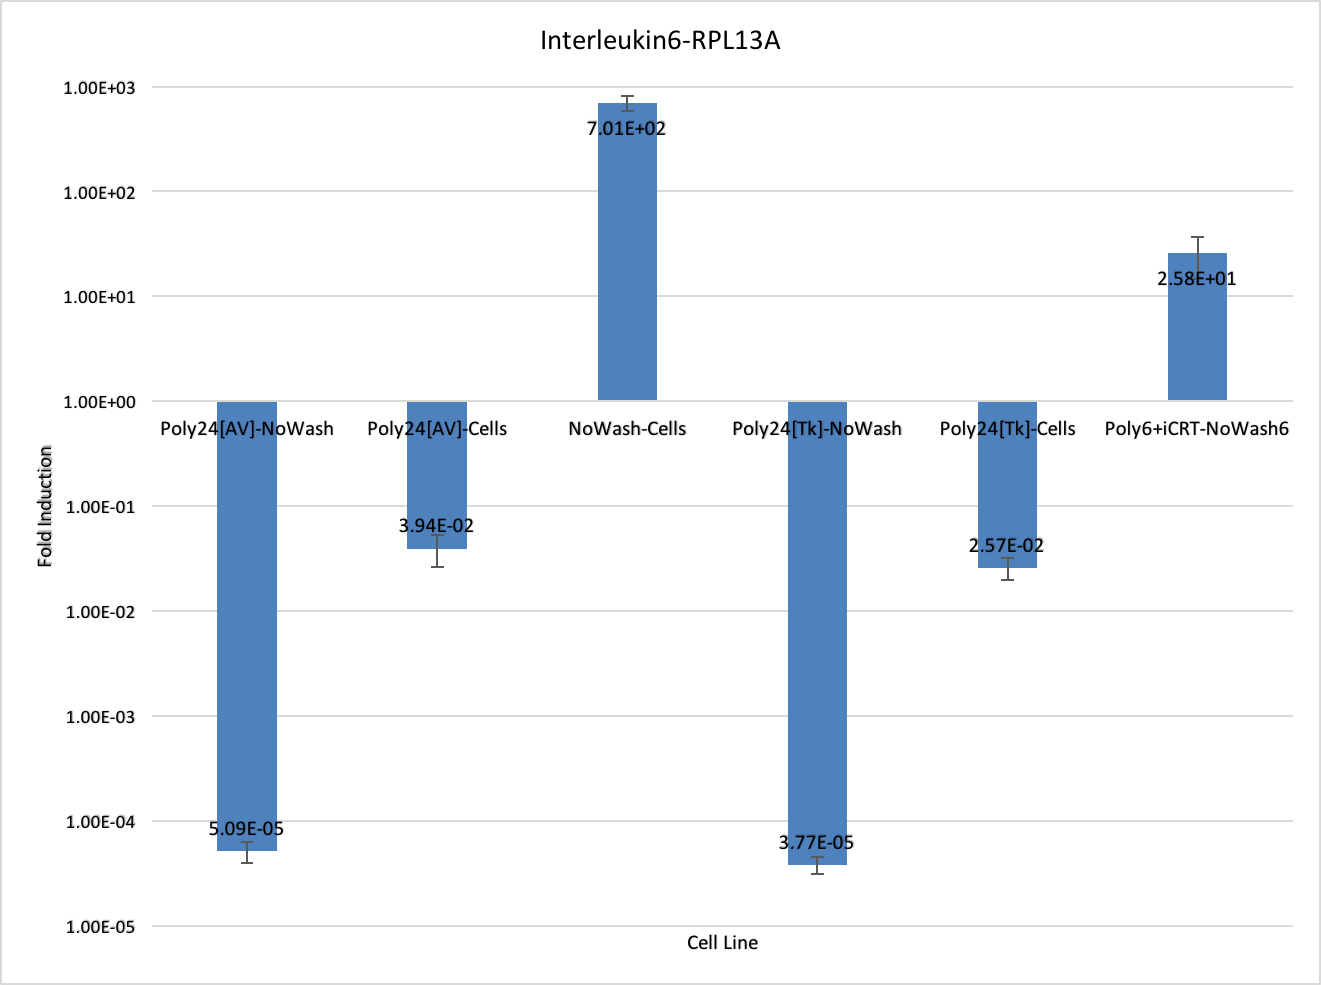
\includegraphics[width=8cm]{il6-rpl13a}
    \caption{Logarithmic fold Inductions for Interleukin-6 vs RPL13A.
    Refer to the analysis subsection of the methods section for insight on how this graph was constructed.
    }
    \label{fig:mesh1}
  \end{figure}

  \begin{figure}[t]
    \centering
    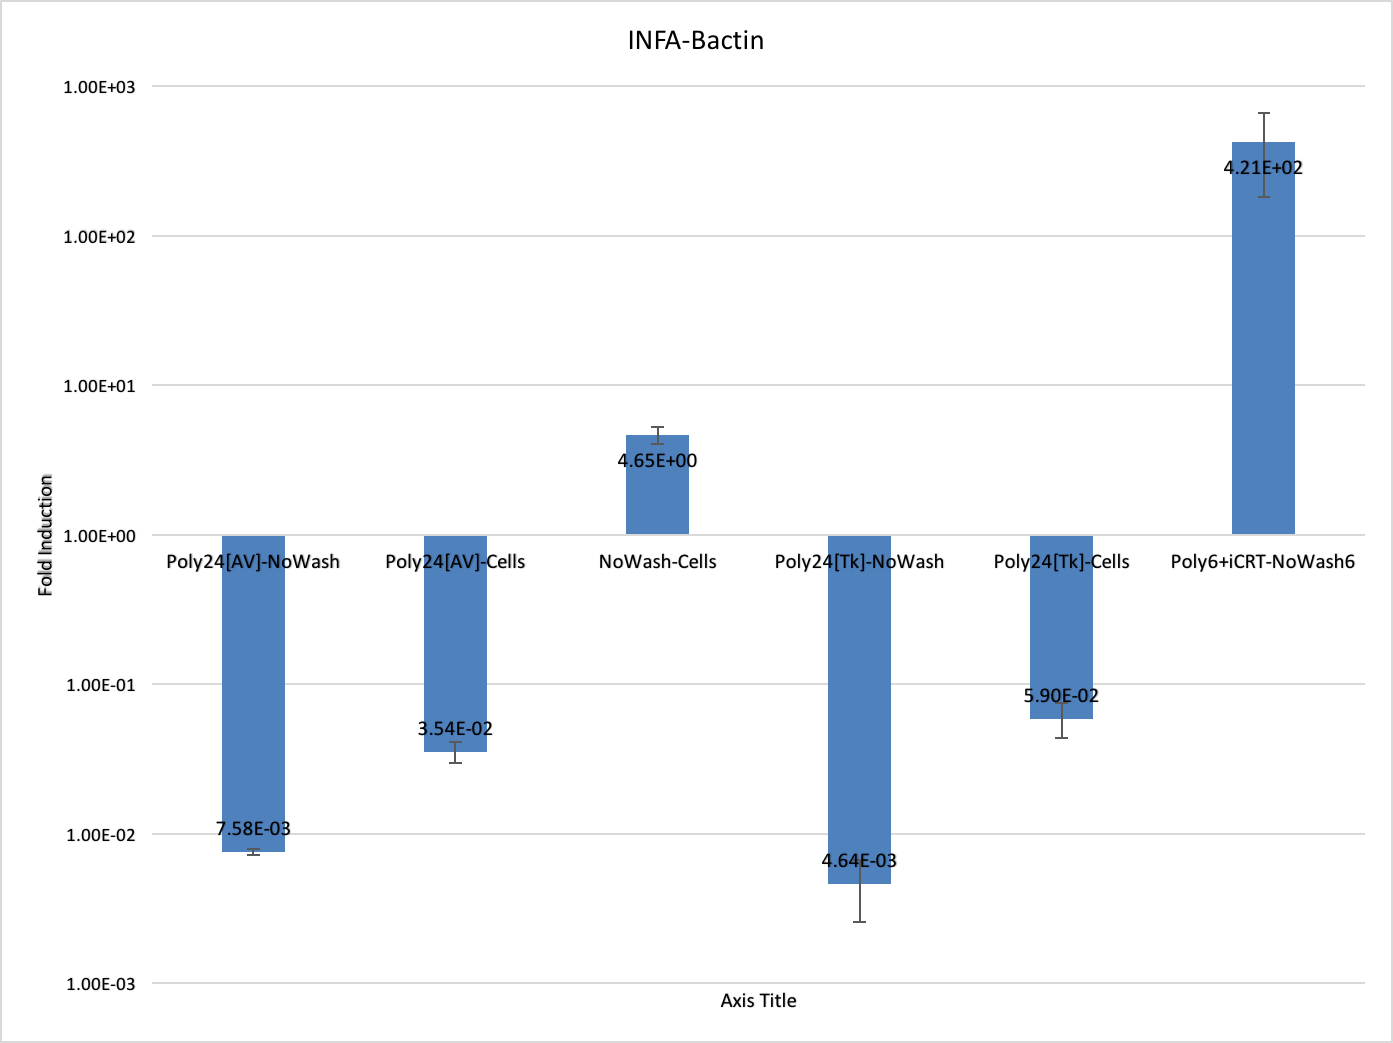
\includegraphics[width=8cm]{infa-bactin}
    \caption{Logarithmic fold Inductions for Interferon-$\alpha$ vs $\beta$-actin.
    Refer to the analysis subsection of the methods section for insight on how this graph was constructed.
    }
    \label{fig:mesh1}
  \end{figure}

  \begin{figure}[t]
    \centering
    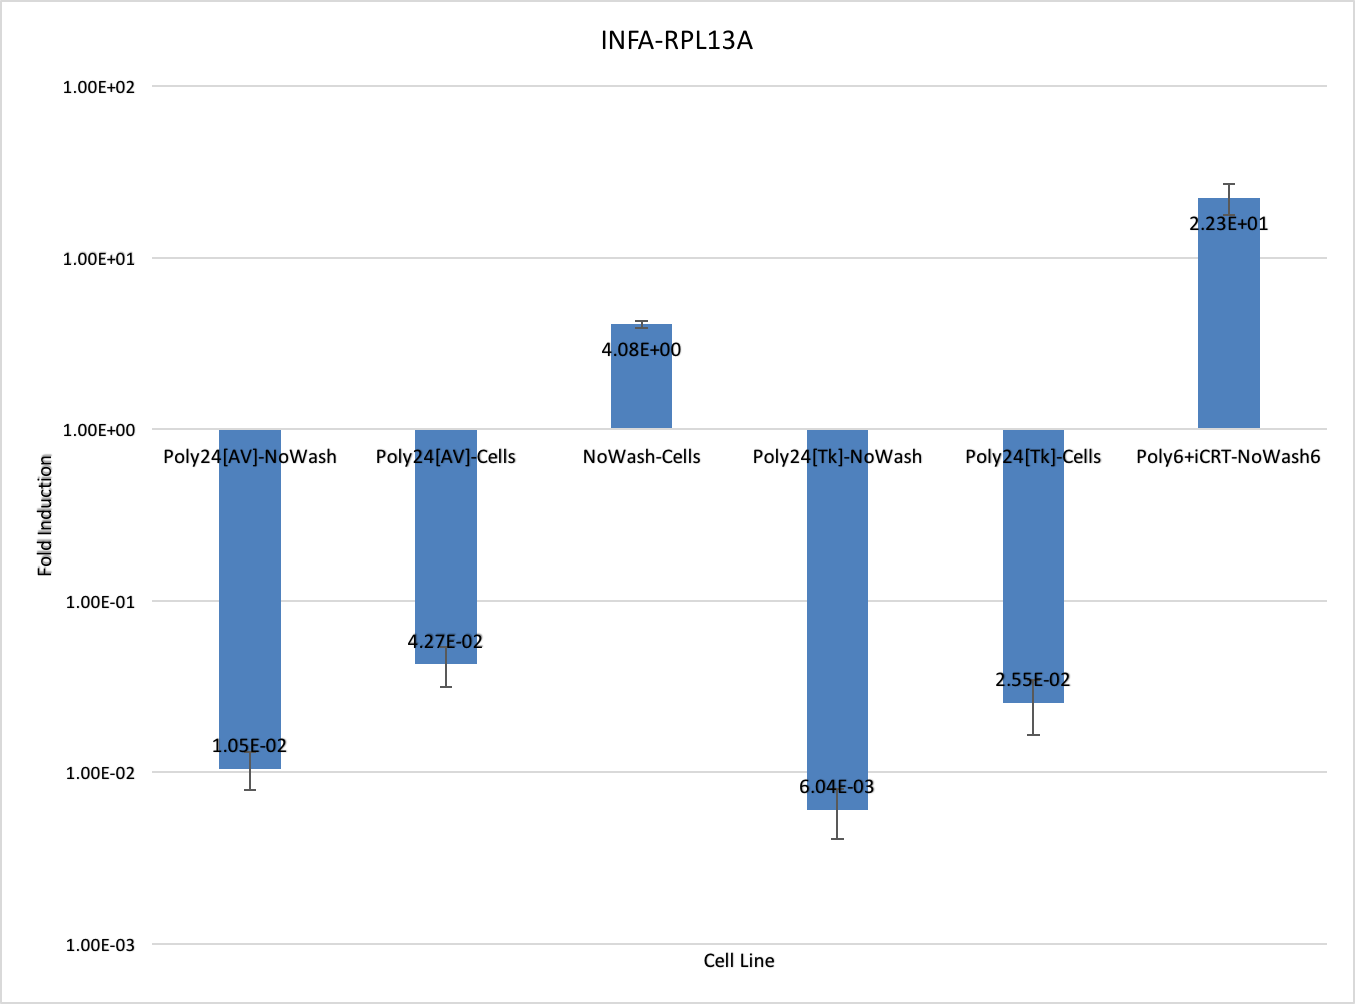
\includegraphics[width=8cm]{infa-rpl13a}
    \caption{
    Logarithmic fold Inductions for Interferon-$\alpha$ an immune cytokine vs RPL13A a standard protien.
    Refer to the analysis subsection of the methods section for insight on how this graph was constructed.
    }
    \label{fig:mesh1}
  \end{figure}

% Now we need a bibliography:
\begin{thebibliography}{5}
    %Each item starts with a \bibitem{reference} command and the details thereafter.
    \bibitem{HOP96} % Transaction paper
    J.~Hagenauer, E.~Offer, and L.~Papke. Iterative decoding of binary block
    and convolutional codes. {\em IEEE Trans. Inform. Theory},
    vol.~42, no.~2, pp.~429–-445, Mar. 1996.

    \bibitem{MJH06} % Conference paper
    T.~Mayer, H.~Jenkac, and J.~Hagenauer. Turbo base-station cooperation for intercell interference cancellation. {\em IEEE Int. Conf. Commun. (ICC)}, Istanbul, Turkey, pp.~356--361, June 2006.

    \bibitem{Proakis} % Book
    J.~G.~Proakis. {\em Digital Communications}. McGraw-Hill Book Co.,
    New York, USA, 3rd edition, 1995.

    \bibitem{talk} % Web document
    F.~R.~Kschischang. Giving a talk: Guidelines for the Preparation and Presentation of Technical Seminars.
    \url{http://www.comm.toronto.edu/frank/guide/guide.pdf}.

    \bibitem{5}
    IEEE Transactions \LaTeX and Microsoft Word Style Files.
    \url{http://www.ieee.org/web/publications/authors/transjnl/index.html}

%http://www.ncbi.nlm.nih.gov/pmc/articles/PMC2143693/pdf/9144766.pdf
%http://www.molbiolcell.org/content/22/21/4047.full.pdf+html?with-ds=yes

%    @Article{Gabay2006,
%    author="Gabay, Cem",
%    title="Interleukin-6 and chronic inflammation",
%    journal="Arthritis Research {\&} Therapy",
%    year="2006",
%    volume="8",
%    number="2",
%    pages="1--6",
%    abstract="Interleukin (IL)-6 is produced at the site of inflammation and plays a key role in the acute phase response as defined by a variety of clinical and biological features such as the production of acute phase proteins. IL-6 in combination with its soluble receptor sIL-6R$\alpha$, dictates the transition from acute to chonic inflammation by changing the nature of leucocyte infiltrate (from polymorphonuclear neutrophils to monocyte/macrophages). In addition, IL-6 exerts stimulatory effects on T- and B-cells, thus favoring chronic inflammatory responses. Strategies targeting IL-6 and IL-6 signaling led to effective prevention and treatment of models of rheumatoid arthritis and other chronic inflammatory diseases.",
%    issn="1478-6354",
%    doi="10.1186/ar1917",
%    url="http://dx.doi.org/10.1186/ar1917"
%    }

\end{thebibliography}

% Your document ends here!
\end{document}
